\section{The pretraining campaign}
\label{sec:pretraining}

\subsection{Setup}

The model was trained on ClimbMix, a 400B-token filtered web corpus,
streamed and tokenized on the fly with a 50k-document shuffle buffer and
a 1\% held-out validation split. Hardware was a TPU v4-64 slice --- 32
chips across 8 hosts --- in pure data parallelism: per-device batch 8 at
sequence length 2048 gives
\begin{equation}
32 \times 8 \times 2048 = 524{,}288 \text{ tokens per optimizer step},
\end{equation}
and the 700{,}000-step budget totals $3.67\times10^{11}$ \emph{step
tokens}. Because the data stream restarts on resume (and the resumed
leg re-streams from a fresh shuffle), unique-token exposure is
$\sim$341B --- the final 26B of step tokens revisit the corpus head.
Throughput held at a median of 1.092M tokens/s (480 ms/step,
Fig.~\ref{fig:throughput}); against the v4 chip's nominal bf16 peak
this is a parameter-FLOP utilization of
\begin{equation}
\frac{6 \, N \, R}{32 \cdot 275\,\mathrm{TF}}
= \frac{6 \cdot 3.077\times10^{8} \cdot 1.092\times10^{6}}
       {8.8\times10^{15}} \approx 23\%,
\end{equation}
a lower bound that ignores all sequence-mixing FLOPs. Holdout loss was
evaluated every 2{,}500 steps and a ten-task lm-eval round ran on-device
every $\sim$20k steps, giving the campaign a benchmark trajectory, not
just an endpoint (Fig.~\ref{fig:evaltraj}).

\begin{figure}[t]
\centering
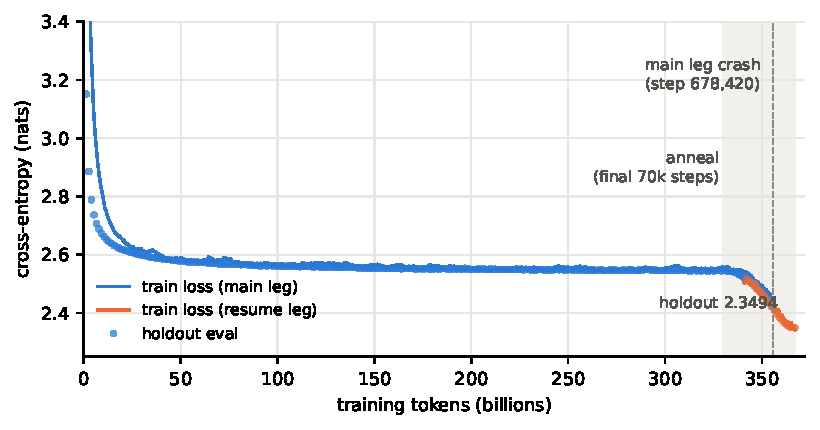
\includegraphics[width=\textwidth]{figures/pretrain_loss.pdf}
\caption{The campaign in one curve: train loss (smoothed) and holdout
evaluations for both W\&B legs against total training tokens. The
shaded band is the terminal anneal; the dashed line marks the main
leg's crash at step 678{,}420. The resume leg (orange) retraces the
main leg's trajectory through the overlap region before extending it
to 367B tokens and holdout 2.3494.}
\label{fig:loss}
\end{figure}

\subsection{Schedule and anneal}

The learning rate followed \eqref{eq:schedule}: brief warmup, then a
constant $2\times10^{-3}$ for 90\% of the run, then cosine to zero over
the final 70k steps (Fig.~\ref{fig:lr}). The anneal is where the
campaign cashed in: holdout fell from 2.5446 (step 620k, pre-anneal) to
2.3494 --- $-0.195$ nats, roughly the same improvement as the preceding
300k constant-rate steps combined --- and every benchmark in the
trajectory bent visibly upward through the shaded region of
Fig.~\ref{fig:evaltraj} (HellaSwag $49.3 \to 56.9$, Lambada
$40.4 \to 47.4$ over the final 80k steps). The benchmark curve was still
rising at step 700k; the budget, not convergence, ended the run.

\begin{figure}[t]
\centering
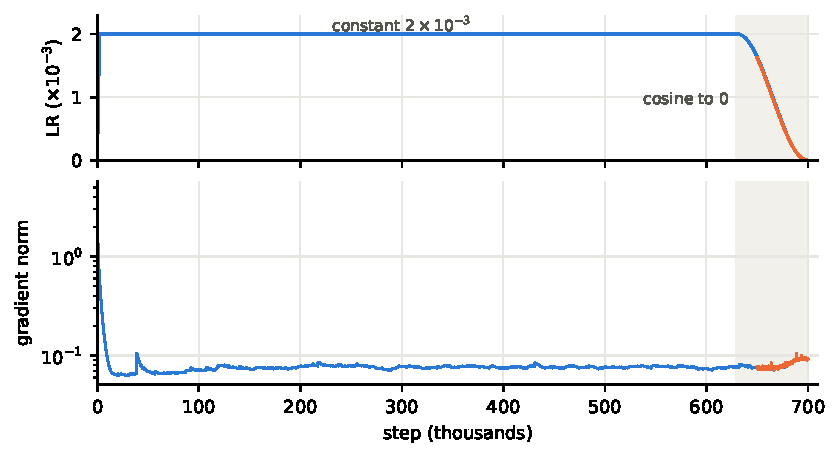
\includegraphics[width=\textwidth]{figures/lr_gradnorm.pdf}
\caption{Learning-rate schedule (top) and smoothed gradient norm
(bottom, log scale) across both legs. The resume leg's schedule
overlays the main leg's exactly through the overlap --- the optimizer
restored to the same trajectory. The gradient norm is flat at
$\sim$0.07 for the entire constant-rate phase; no clipping events, no
spikes, no drift.}
\label{fig:lr}
\end{figure}

\begin{figure}[t]
\centering
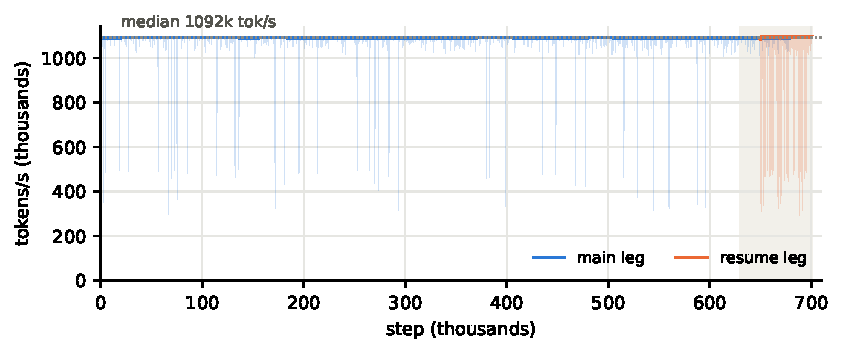
\includegraphics[width=\textwidth]{figures/throughput.pdf}
\caption{Slice throughput over the campaign (rolling median over raw
per-step rates; faint traces show the raw series, whose dips are eval
and checkpoint pauses). The line is flat at 1.09M tokens/s for four
days of wall time --- the data pipeline, running host-side over
streamed HF shards, never became the bottleneck.}
\label{fig:throughput}
\end{figure}

\subsection{The crash, and what a clean resume looks like}

At step 678{,}420 --- 22k steps from the finish, inside the anneal ---
the main leg died (W\&B state \emph{crashed}; the slice itself
survived). Training resumed three days later from the most recent
durable checkpoint ($\approx$ step 650k) as a second W\&B leg,
re-running steps 650k--700k with a restarted data stream.

The resume's fidelity is measurable rather than assumed, three ways.
First, the loss curves: through the 28k-step overlap the resumed leg
retraces the original to within smoothing width (Fig.~\ref{fig:loss}).
Second, the schedule: the resumed learning-rate curve lands exactly on
the original cosine (Fig.~\ref{fig:lr}). Third, the benchmark round at
step 660k, which both legs executed, agreed within noise (HellaSwag
$51.9$ vs.\ $51.3$, ARC-e $63.0$ vs.\ $62.7$) despite the different
shuffle --- the model state, not the data order, determines the
trajectory at this point in training. The campaign's conclusion is
thereby independent of the crash: the final 700k-step model is the same
model the uninterrupted run would have produced, up to data-order noise
that the 660k A/B bounds at a few tenths of a point.

\begin{figure}[t]
\centering
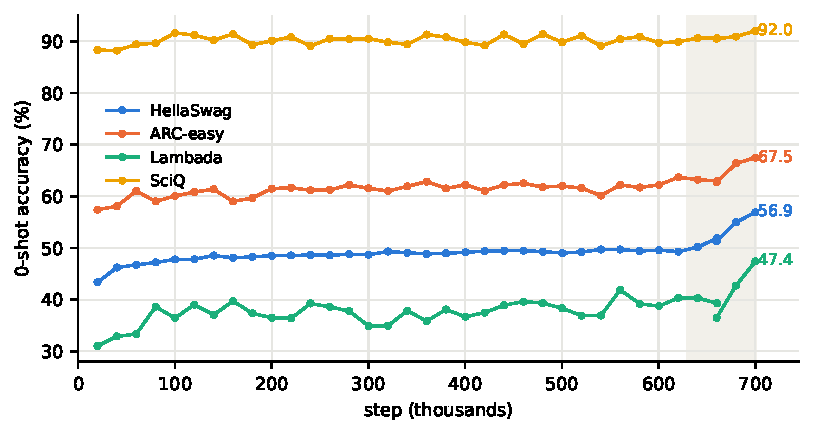
\includegraphics[width=\textwidth]{figures/eval_trajectory.pdf}
\caption{In-training 0-shot benchmark trajectory (both legs), one
lm-eval round per $\sim$20k steps. Long plateaus through the
constant-rate phase, then the anneal (shaded) lifts every task
simultaneously --- the argument, in one figure, for spending the last
10\% of any fixed budget on a terminal anneal.}
\label{fig:evaltraj}
\end{figure}
